\documentclass[11pt,a4paper]{article}

\usepackage[utf8]{inputenc}
\usepackage{url}
\usepackage[margin=1in]{geometry}
\usepackage{graphicx}

\title{GitHub Cheat Sheet}
\date{}
\author{Econ 213R - Applied Machine Learning}

\begin{document}
\vspace*{-75pt}
    {\let\newpage\relax\maketitle}
    
\section*{What is GitHub?}
\begin{itemize}
\item Explain idea of GitHub
\item Define ``repository"
\item Define ``fork", ``clone", ``commit", ``push/pull"
\item Explain what a README is
\end{itemize}
    
\section*{Register for GitHub}
First, you need to make an account with GitHub.
Go to \url{www.github.com}. 
Sign up from the home page with any email and username you want.
Follow the initial signup steps.
Note that private repositories require monthly payments; however, you can have an unlimited number of public repositories for free.
Once you are done signing up, you are ready to create and fork repositories.

\section*{Creating Repositories}
Navigate to your GitHub profile.
It should look something like Figure \ref{fig:init-prof}.

\begin{figure}[h]
\centering
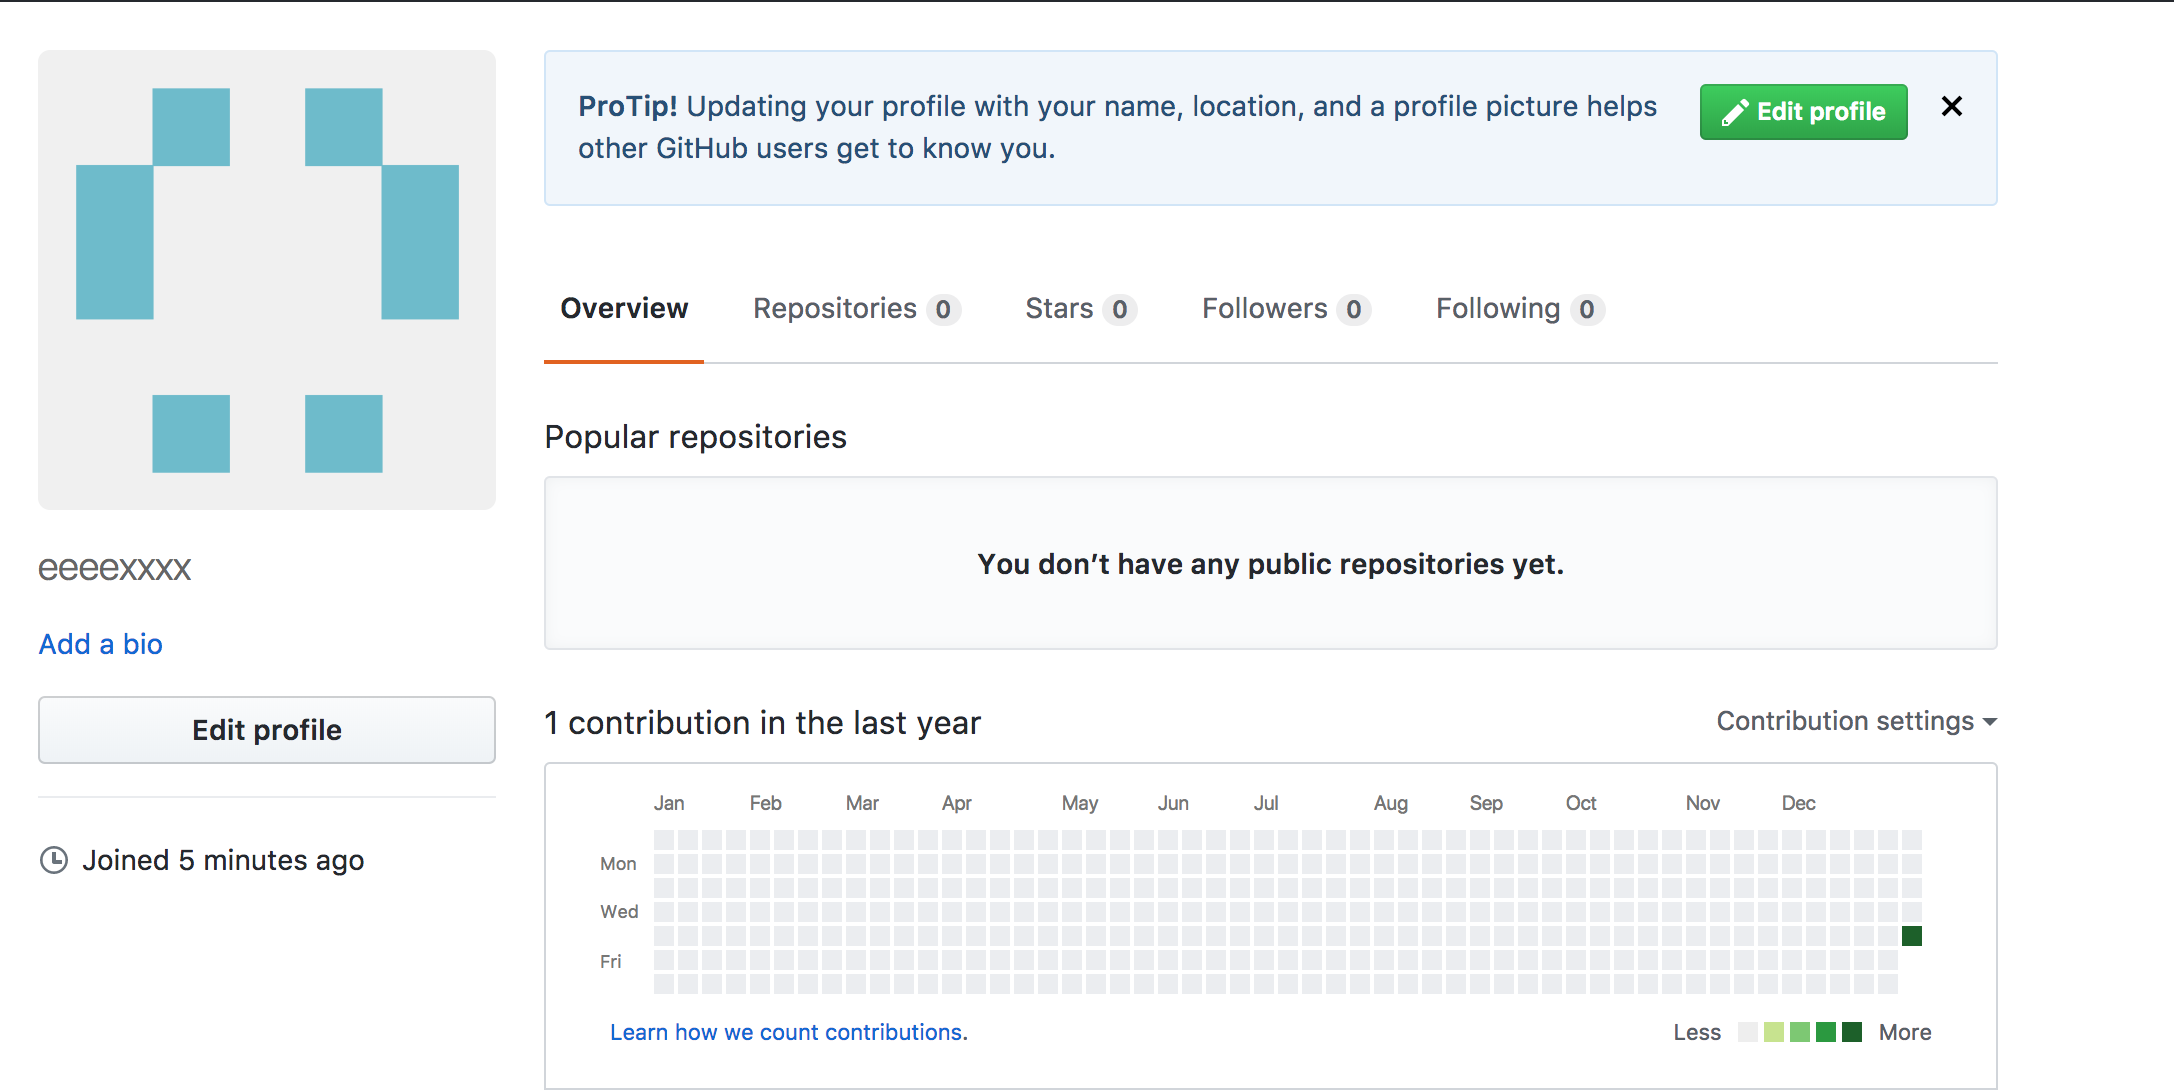
\includegraphics[width=.7\textwidth]{figures/init_profile.png}
\caption{Profile Screen}
\label{fig:init-prof}
\end{figure}

Click the ``Repositories" tab.
Click the button that says ``New" (see Figure \ref{fig:repo}).

\begin{figure}[h]
\centering
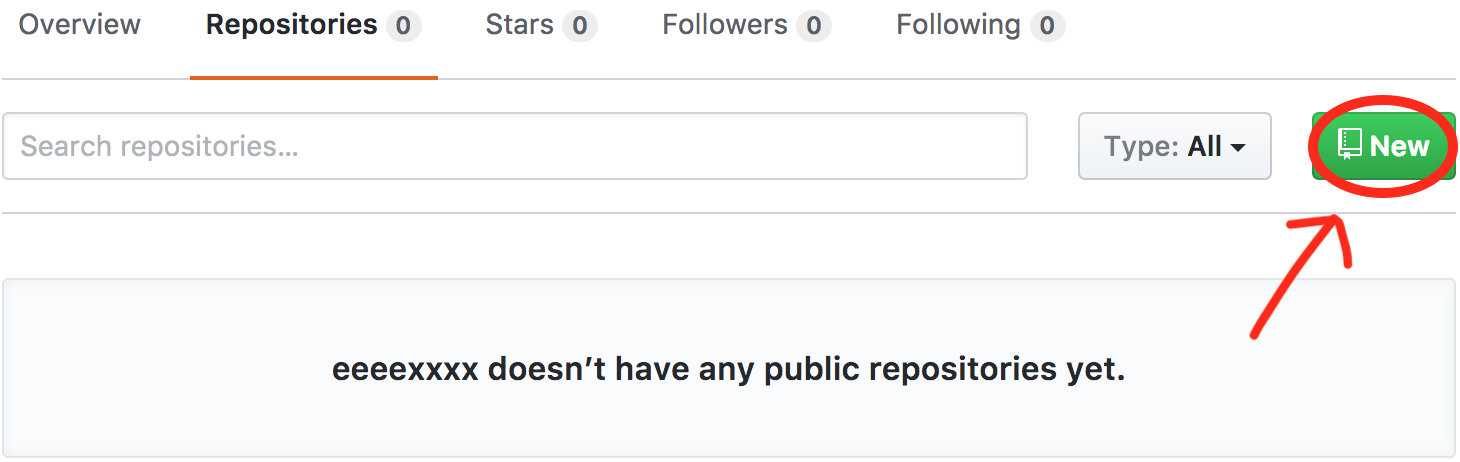
\includegraphics[width=.7\textwidth]{figures/repository_page.png}
\caption{Repository Screen}
\label{fig:repo}
\end{figure}


\section*{Forking Repositories}
Navigate to the class repository. 
The link is \url{https://github.com/tfolkman/byu_econ_applied_machine_learning}.

\section*{Using Command Line}
\subsection*{Making Changes}

\subsection*{Committing Changes}

\subsection*{Pulling Changes}

\section*{Using the Website}
\subsection*{Downloading Files}

\subsection*{Uploading Files}

\end{document}